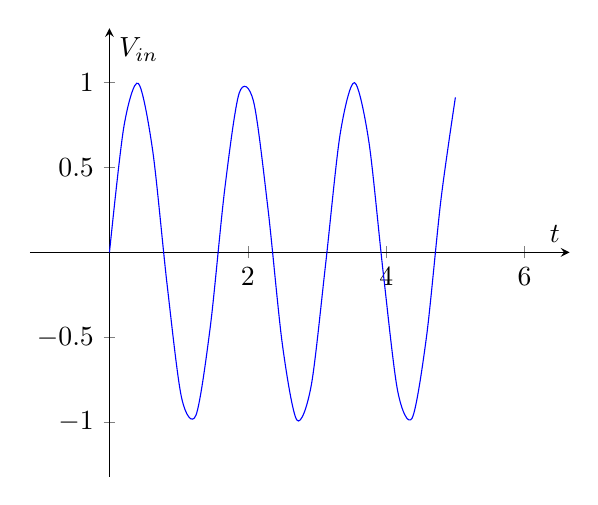
\begin{tikzpicture}
    \begin{axis}[
        domain=0:5,
        axis lines = middle,
        xmin = -0.5,
        xmax = 6,
        ymin = -1.1,
        ymax = 1.1,
        xlabel = $t$,
        ylabel = $V_{in}$,
        enlargelimits = true,
    ]
        \addplot[smooth,mark=none,color=blue] {sin(4*deg(x))};
    \end{axis}
\end{tikzpicture}
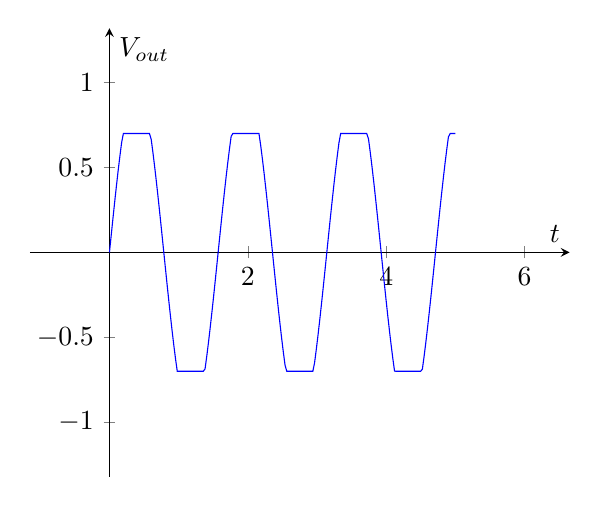
\begin{tikzpicture}
    \begin{axis}[
        domain=0:5,
        axis lines = middle,
        xmin = -0.5,
        xmax = 6,
        ymin = -1.1,
        ymax = 1.1,
        xlabel = $t$,
        ylabel = $V_{out}$,
        enlargelimits = true,
        y filter/.expression={y > 0.7 ? 0.7 : (y < -0.7 ? -0.7 : y)},
    ]
        \addplot[samples=200,mark=none,color=blue] {sin(4*deg(x))};
    \end{axis}
\end{tikzpicture}
